\documentclass[11pt,a4paper,twoside]{article}

% ── Encoding ──────────────────────────────────────────────────────────────────
\usepackage[utf8]{inputenc}
\usepackage[T1]{fontenc}
\usepackage[portuguese]{babel}

% ── Typography ────────────────────────────────────────────────────────────────
\usepackage{mathpazo}
\usepackage[scaled=0.90]{helvet}
\usepackage[activate={true,nocompatibility},final,tracking=true,kerning=true,expansion=false]{microtype}

% ── Layout ────────────────────────────────────────────────────────────────────
\usepackage[
  a4paper,
  top=3.0cm, bottom=3.2cm,
  inner=2.8cm, outer=2.4cm,
  headsep=1.0cm,
  footskip=1.2cm
]{geometry}

% ── Colors ────────────────────────────────────────────────────────────────────
\usepackage[table,dvipsnames]{xcolor}
\definecolor{INK}{HTML}{1A1A2E}
\definecolor{RULE}{HTML}{1856B8}
\definecolor{ACCENT}{HTML}{0C2A59}
\definecolor{MUTED}{HTML}{5C6475}
\definecolor{ROWSHADE}{HTML}{F4F6FA}
\definecolor{TAGHI}{HTML}{1856B8}
\definecolor{TAGMED}{HTML}{E07B00}
\definecolor{TAGLO}{HTML}{2E7D32}
\definecolor{TAGNEUTRAL}{HTML}{4A5568}
\definecolor{BOXBG}{HTML}{EEF2FA}
\definecolor{BOXLINE}{HTML}{1856B8}

% ── Graphics ──────────────────────────────────────────────────────────────────
\usepackage{graphicx}

% ── Tables ────────────────────────────────────────────────────────────────────
\usepackage{booktabs}
\usepackage{longtable}
\usepackage{tabularx}
\usepackage{array}
\usepackage{multirow}
\usepackage{makecell}
\renewcommand{\arraystretch}{1.38}
\setlength{\tabcolsep}{3.5pt}
\newcolumntype{Y}{>{\raggedright\arraybackslash}X}
\newcolumntype{C}{>{\centering\arraybackslash}X}
\newcolumntype{R}{>{\raggedleft\arraybackslash}X}

% ── Lists ─────────────────────────────────────────────────────────────────────
\usepackage{enumitem}
\setlist{
  leftmargin=1.5em,
  itemsep=2pt,
  topsep=4pt,
  parsep=0pt
}
\setlist[itemize,1]{label=\textcolor{RULE}{\rule[0.35ex]{4pt}{4pt}}}
\setlist[itemize,2]{label=\textcolor{MUTED}{\textendash}}
\setlist[enumerate,1]{label=\textcolor{RULE}{\arabic*.}}

% ── Section Titles ────────────────────────────────────────────────────────────
\usepackage{titlesec}
\titleformat{\section}
  {\sffamily\bfseries\large\color{RULE}}
  {\thesection}
  {0.8em}
  {}
  [\vspace{1pt}{\color{RULE}\titlerule[0.8pt]}\vspace{4pt}]

\titleformat{\subsection}
  {\sffamily\bfseries\normalsize\color{ACCENT}}
  {\thesubsection}
  {0.7em}
  {}

\titleformat{\subsubsection}
  {\itshape\normalsize\color{ACCENT}}
  {}
  {0em}
  {}

\titlespacing*{\section}      {0pt}{20pt}{8pt}
\titlespacing*{\subsection}   {0pt}{14pt}{4pt}
\titlespacing*{\subsubsection}{0pt}{10pt}{2pt}

% ── Headers / Footers ─────────────────────────────────────────────────────────
\usepackage{fancyhdr}
\usepackage{lastpage}
\pagestyle{fancy}
\fancyhf{}
\fancyhead[LE,RO]{\small\sffamily\color{MUTED}Ponto de Controlo 3 - SMARTER HUB}
\fancyhead[RE,LO]{\small\sffamily\color{MUTED}PROES 2025/2026}
\fancyfoot[C]{\small\sffamily\color{MUTED}\thepage\,/\,\pageref{LastPage}}
\renewcommand{\headrulewidth}{0.4pt}
\renewcommand{\headrule}{\color{RULE!40}\hrule height 0.4pt \vspace{0pt}}
\renewcommand{\footrulewidth}{0pt}

% ── Boxes / Callouts ──────────────────────────────────────────────────────────
\usepackage[most]{tcolorbox}
\tcbuselibrary{skins, breakable}

\newtcolorbox{callout}[1][]{
  enhanced, breakable,
  colback=BOXBG, colframe=BOXLINE,
  boxrule=0pt, leftrule=3pt,
  arc=0pt, outer arc=0pt,
  left=10pt, right=10pt, top=7pt, bottom=7pt,
  fontupper=\small,
  #1
}

\newtcolorbox{note}[1][]{
  enhanced, breakable,
  colback=ROWSHADE, colframe=MUTED!40,
  boxrule=0pt, leftrule=2pt,
  arc=0pt,
  left=10pt, right=8pt, top=5pt, bottom=5pt,
  fontupper=\small\color{MUTED},
  #1
}

% ── Table helpers ─────────────────────────────────────────────────────────────
\newcommand{\tH}[1]{\textbf{\sffamily\small\color{white}#1}}
\newcommand{\theadrow}{\rowcolor{ACCENT}}

% ── Misc ──────────────────────────────────────────────────────────────────────
\usepackage{setspace}
\usepackage{parskip}
\setlength{\parskip}{5pt}
\setlength{\parindent}{0pt}
\usepackage{hyperref}
\hypersetup{
  colorlinks=true,
  linkcolor=RULE,
  urlcolor=RULE,
  citecolor=RULE,
  pdftitle={SMARTER HUB - Ponto de Controlo 3 - Versão Enxuta},
  pdfauthor={Patrick Costa}
}
\usepackage{eso-pic}

\begin{document}
\setstretch{1.18}

\begin{titlepage}
\thispagestyle{empty}
 \AddToShipoutPictureBG*{%
   \includegraphics[width=\paperwidth,height=\paperheight]{capa_pc3.png}%
 }
 \vspace*{\fill}
\end{titlepage}
\nopagecolor

\tableofcontents
\newpage

\section{Identificação}

\textbf{Aluno:} Patrick Dias Mendes da Costa\\
\textbf{Supervisor:} Camila Teixeira\\
\textbf{Orientador:} Marílio Cardoso\\
\textbf{Entidade acolhedora:} Tlantic Portugal - Sistemas de Informação, S.A.\\
\textbf{Local e modo:} Rua Manuel Pinto de Azevedo, n626, 1.º Piso, 4100-320, Porto; regime híbrido

\section{Alterações Significativas ao Plano Inicial}

\subsection{Logística}
\begin{itemize}
  \item Sem alteração de local, entidade, orientação ou regime de trabalho.
  \item Manteve-se o modelo de acompanhamento académico e de negócio definido no arranque.
\end{itemize}

\subsection{Objetivos gerais e específicos}
\begin{itemize}
  \item O objetivo geral mantém-se: consolidar processos de pessoas numa única plataforma com rastreabilidade e governação de acesso.
  \item O escopo do checkpoint foi ampliado com entregas efetivas em banco de horas BR, admissões, plano de carreira e internacionalização.
\end{itemize}

\subsection{Plano}
\rowcolors{1}{ROWSHADE}{white}
\begin{longtable}{>{\small\bfseries}p{4.8cm} >{\small\centering\arraybackslash}p{2.4cm} >{\small\centering\arraybackslash}p{1.7cm} >{\small}p{5.3cm}}
\theadrow
\tH{Bloco} & \tH{Janela temporal} & \tH{Estado} & \tH{Leitura no PC3} \\
\midrule
\endfirsthead
\theadrow
\tH{Bloco} & \tH{Janela temporal} & \tH{Estado} & \tH{Leitura no PC3} \\
\midrule
\endhead
Iniciação e arranque & 07/04 -- 15/04 & 100\% & Fechado no prazo \\
Planeamento inicial & 16/04 -- 01/05 & 100\% & Fechado no prazo \\
Análise, desenho e arquitetura & 22/04 -- 22/05 & 100\% & Fechado no prazo \\
Desenvolvimento do escopo PC3 & 22/04 -- 22/05 & 100\% & Entregas-alvo concluídas \\
Consolidação e fecho & 15/06 -- 03/07 & Planeado & Hardening e refinamento em PC4+ \\
\bottomrule
\end{longtable}

\subsection{Outros ajustes relevantes}
\begin{itemize}
  \item Framing da entrega: \textit{pronto para piloto operacional}, não \textit{produto encerrado}.
  \item Critério de avaliação reforçado por evidência técnica (código, teste e comportamento observável).
\end{itemize}

\section{Análise e Desenho}

\subsection{Objetivo do desenho}
O desenho do PC3 foi construído para garantir uma plataforma coerente, audível e fácil de evoluir. A prioridade não foi apenas fechar funcionalidades, mas estruturar a solução de forma que o comportamento da aplicação seja previsível, rastreável e consistente entre frontend, backend e dados.

\subsection{Estrutura da solução}
\begin{itemize}
  \item \textbf{Frontend}: interface em React/Vite, organizada por páginas funcionais e contexto de sessão/permissões.
  \item \textbf{Backend}: API em Express/TypeScript, responsável por autenticação, regras de negócio e validação por domínio.
  \item \textbf{Dados}: persistência em PostgreSQL via Prisma, com entidades normalizadas para utilizadores, equipas, férias, permissões e banco de horas.
  \item \textbf{Integrações}: geração de PDFs/XLSX, upload de ficheiros e ligação com mecanismos externos de autenticação quando aplicável.
\end{itemize}

\subsection{Decisões de desenho}
\begin{itemize}
  \item O controlo de acesso é baseado em permissões efetivas e escopo, não apenas em papéis de interface.
  \item Os fluxos críticos usam estado explícito e histórico, para preservar rastreabilidade e permitir auditoria.
  \item A lógica de negócio é separada da interface, reduzindo acoplamento e facilitando manutenção e expansão futura.
  \item O modelo foi desenhado para suportar o PC4 sem reestruturar os componentes centrais.
\end{itemize}

\subsection{Diagramas de suporte}
\begin{itemize}
  \item Casos de uso (resumo): visão executiva dos fluxos críticos e dos principais atores (ver Anexo A, Figura~\ref{fig:anexo-casos-uso}).
  \item Arquitetura por componentes (completo): separação detalhada entre interface, API, persistência e integrações (ver Anexo A, Figura~\ref{fig:anexo-arquitetura}).
  \item Modelo de dados essencial (completo): entidades nucleares e relações que sustentam os fluxos do produto (ver Anexo A, Figura~\ref{fig:anexo-modelo-dados}).
\end{itemize}

\begin{callout}
Para manter o corpo principal focado na análise textual, os três diagramas de suporte estão apresentados no \textbf{Anexo A}.
\end{callout}

\begin{callout}
Os diagramas e a implementação estão alinhados: o desenho valida a estrutura da solução e a solução confirma o desenho.
\end{callout}

\section{Evidências de Implementação}

\begin{callout}
Nesta secção a intenção é mostrar a solução em funcionamento. O foco deixa de ser a implementação interna e passa a ser a experiência visível da plataforma: entrada, navegação, consulta de dados e execução dos fluxos principais.
\end{callout}

\rowcolors{1}{ROWSHADE}{white}
\begin{longtable}{>{\small\bfseries}p{3.6cm} >{\small}p{4.9cm} >{\small}p{5.2cm}}
\theadrow
\tH{Área} & \tH{O que mostrar no print} & \tH{Porque é relevante} \\
\midrule
\endfirsthead
\theadrow
\tH{Área} & \tH{O que mostrar no print} & \tH{Porque é relevante} \\
\midrule
\endhead
Entrada na plataforma & Página de login e autenticação concluída & Mostra acesso real e validação de sessão ativa \\
Visão geral & Home/dashboard com informação operacional carregada & Introduz a plataforma e a leitura inicial do utilizador \\
Ficha do colaborador & Página de perfil com dados pessoais e profissionais & Mostra a base de gestão de informação do sistema \\
Férias/Ausências & Fluxo de pedido de férias com estado visível & Evidencia um processo completo do PC3 \\
Permissões & Gestão de permissões por utilizador com histórico & Mostra governação de acesso e auditabilidade \\
Banco de horas BR & Saldo e movimentos de banco de horas & Evidencia regras operacionais regionais já ativas \\
\bottomrule
\end{longtable}

\subsection{Evidências Visuais da Plataforma (prints a incluir)}

\begin{callout}
No PC3 já existe implementação funcional suficiente para demonstrar evidência visual direta da solução. As capturas abaixo são evidências reais da plataforma e devem ser lidas como prova de comportamento observável.
\end{callout}

\rowcolors{1}{ROWSHADE}{white}
\begin{longtable}{>{\small\bfseries}p{2.0cm} >{\small}p{4.1cm} >{\small}p{4.5cm} >{\small}p{3.2cm}}
\theadrow
\tH{ID} & \tH{Ecrã / fluxo a capturar} & \tH{O que a evidência deve provar} & \tH{Estado esperado visível} \\
\midrule
\endfirsthead
\theadrow
\tH{ID} & \tH{Ecrã / fluxo a capturar} & \tH{O que a evidência deve provar} & \tH{Estado esperado visível} \\
\midrule
\endhead
V1 & Página de login e autenticação & Entrada na plataforma e validação de sessão ativa & Login bem-sucedido + utilizador autenticado \\
V2 & Home / dashboard principal & Visão consolidada da plataforma para utilizador autenticado & Página inicial com informação operacional carregada \\
V3 & Ficha de colaborador (perfil) & Disponibilidade da ficha e dados operacionais do utilizador & Dados pessoais/profissionais visíveis para consulta/edição \\
E1 & Pedido de férias & Registo e rastreabilidade de pedido no fluxo de ausências & Pedido apresentado com estado e metadados associados \\
E2 & Gestão de permissões por utilizador & Governação de acesso com permissões explícitas & Permissões listadas com estado e controlo por utilizador \\
E3 & Banco de horas BR & Consulta operacional do saldo e movimentos associados & Saldo e detalhe de lançamentos visíveis \\
\bottomrule
\end{longtable}

\subsection{Galeria de Evidências}

\begin{figure}[htbp]
  \centering
  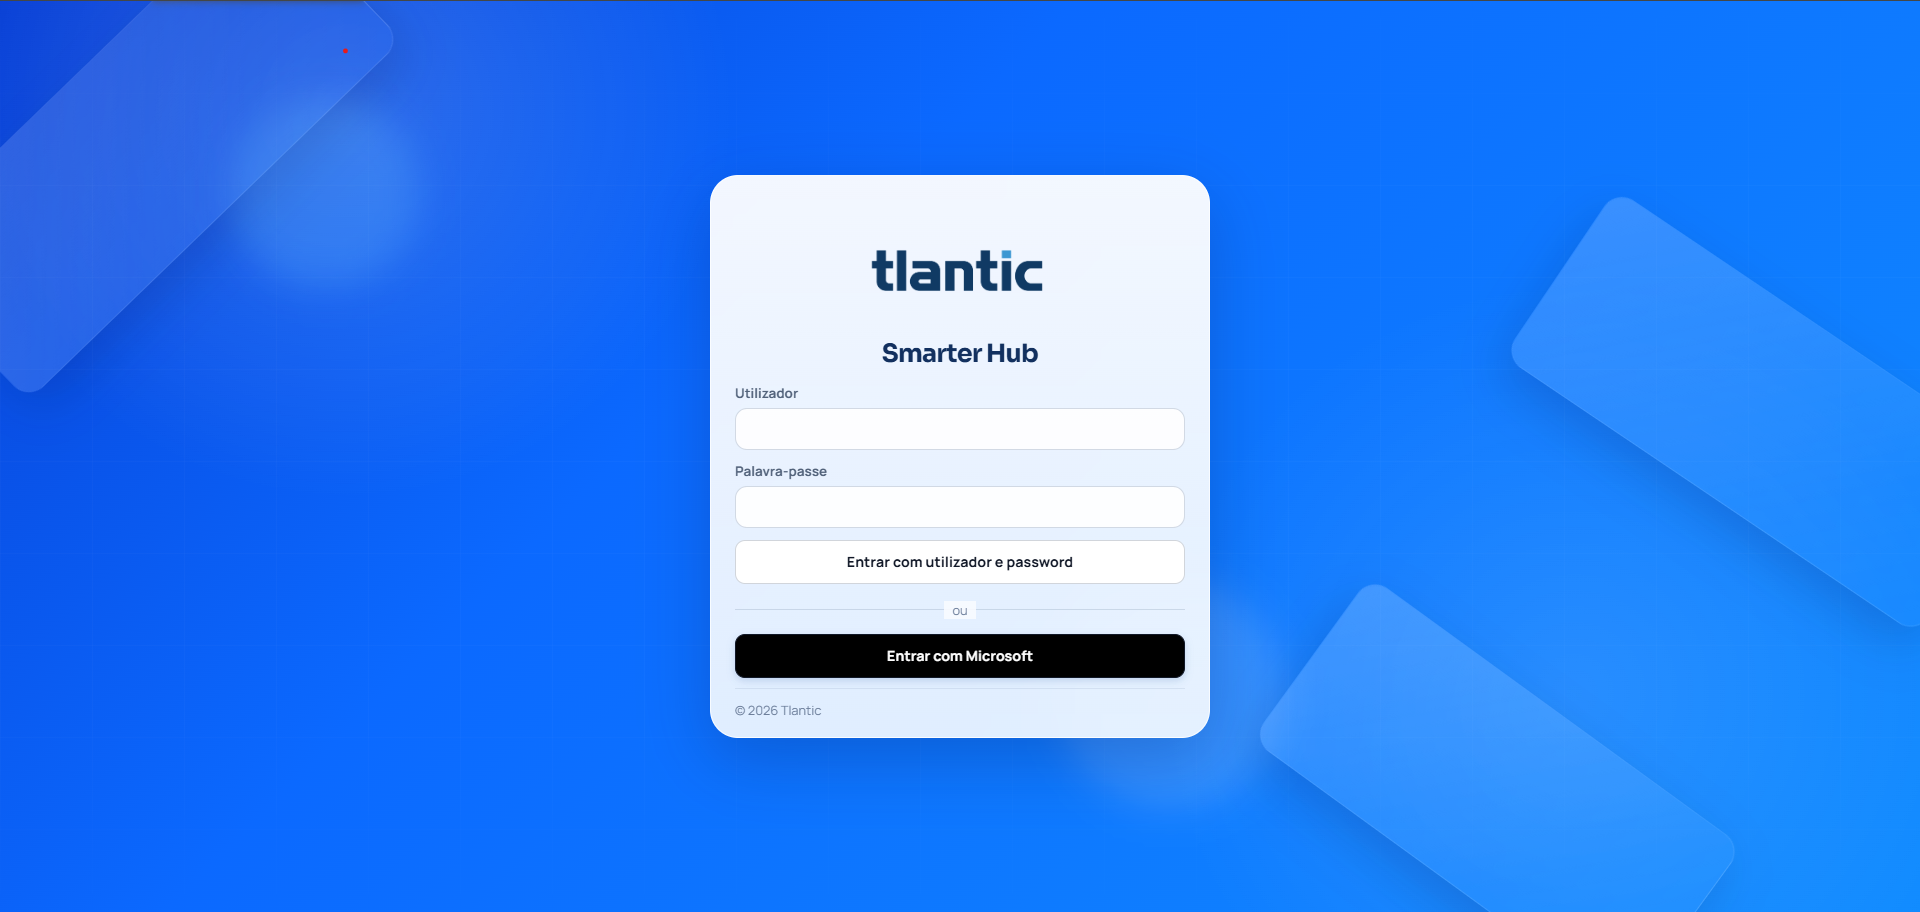
\includegraphics[width=0.94\textwidth]{screenshots/login.png}
  \caption{Evidência V1 - Página de login e autenticação da plataforma.}
\end{figure}

\begin{figure}[htbp]
  \centering
  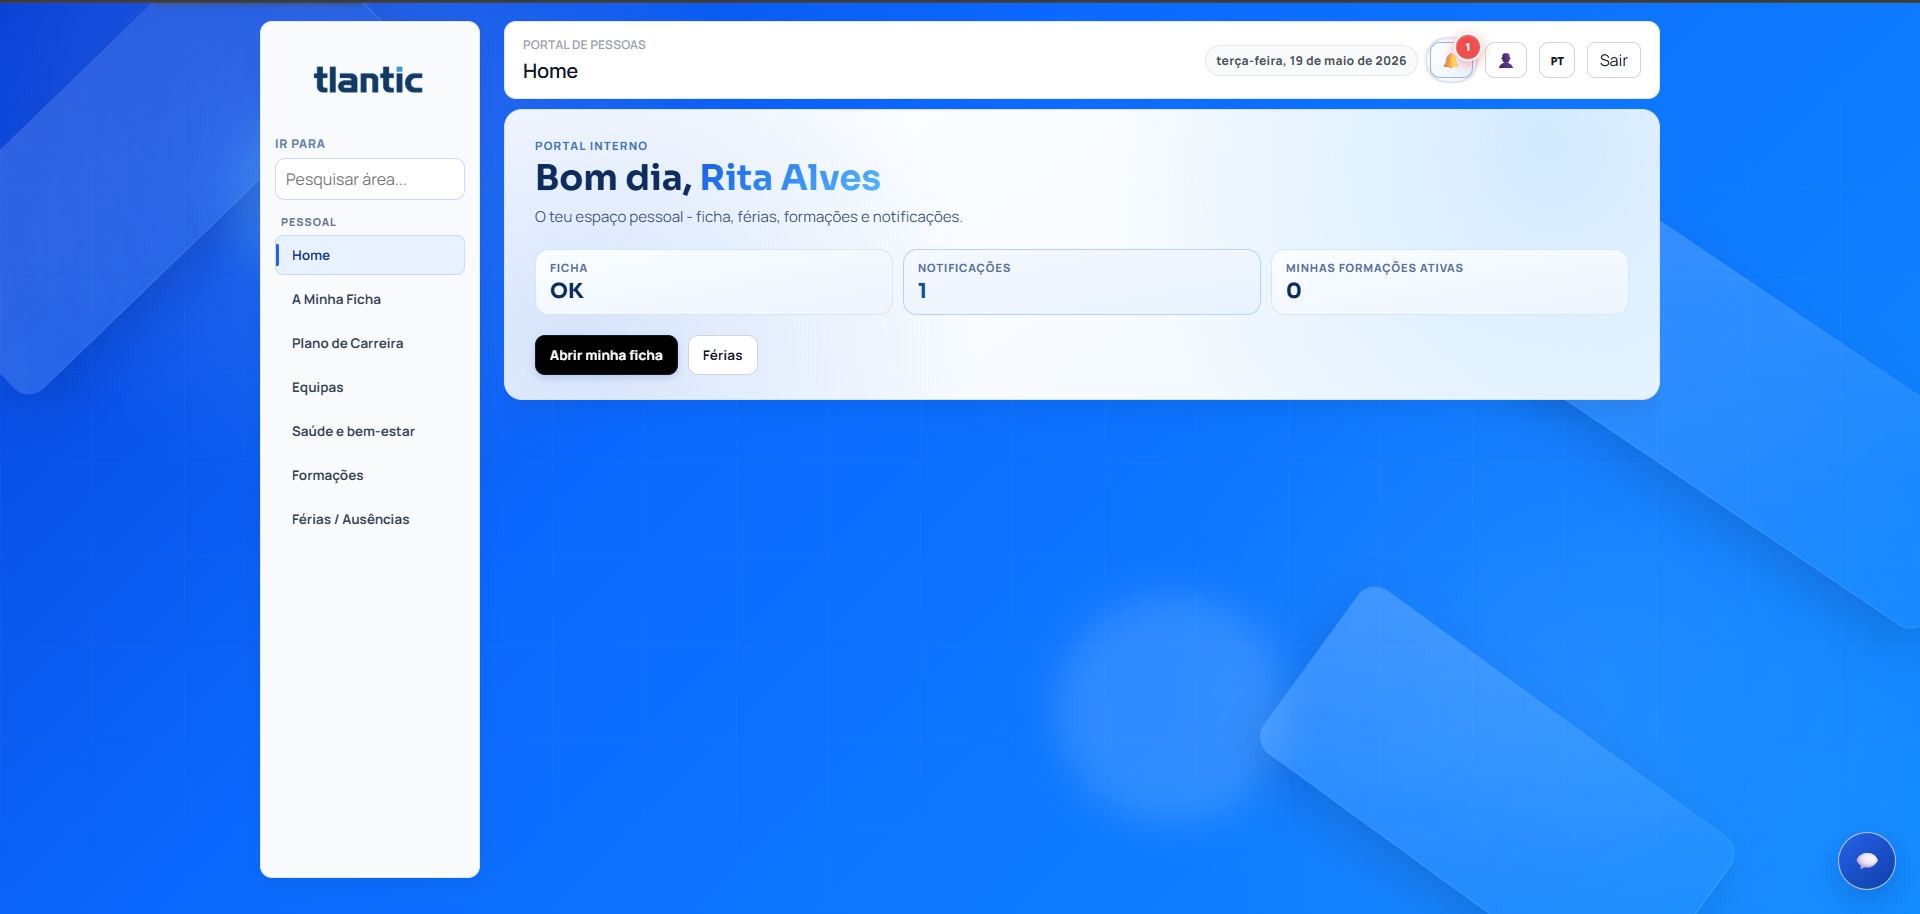
\includegraphics[width=0.94\textwidth]{screenshots/home.png}
  \caption{Evidência V2 - Home/dashboard com visão geral operacional da plataforma.}
\end{figure}

\begin{figure}[htbp]
  \centering
  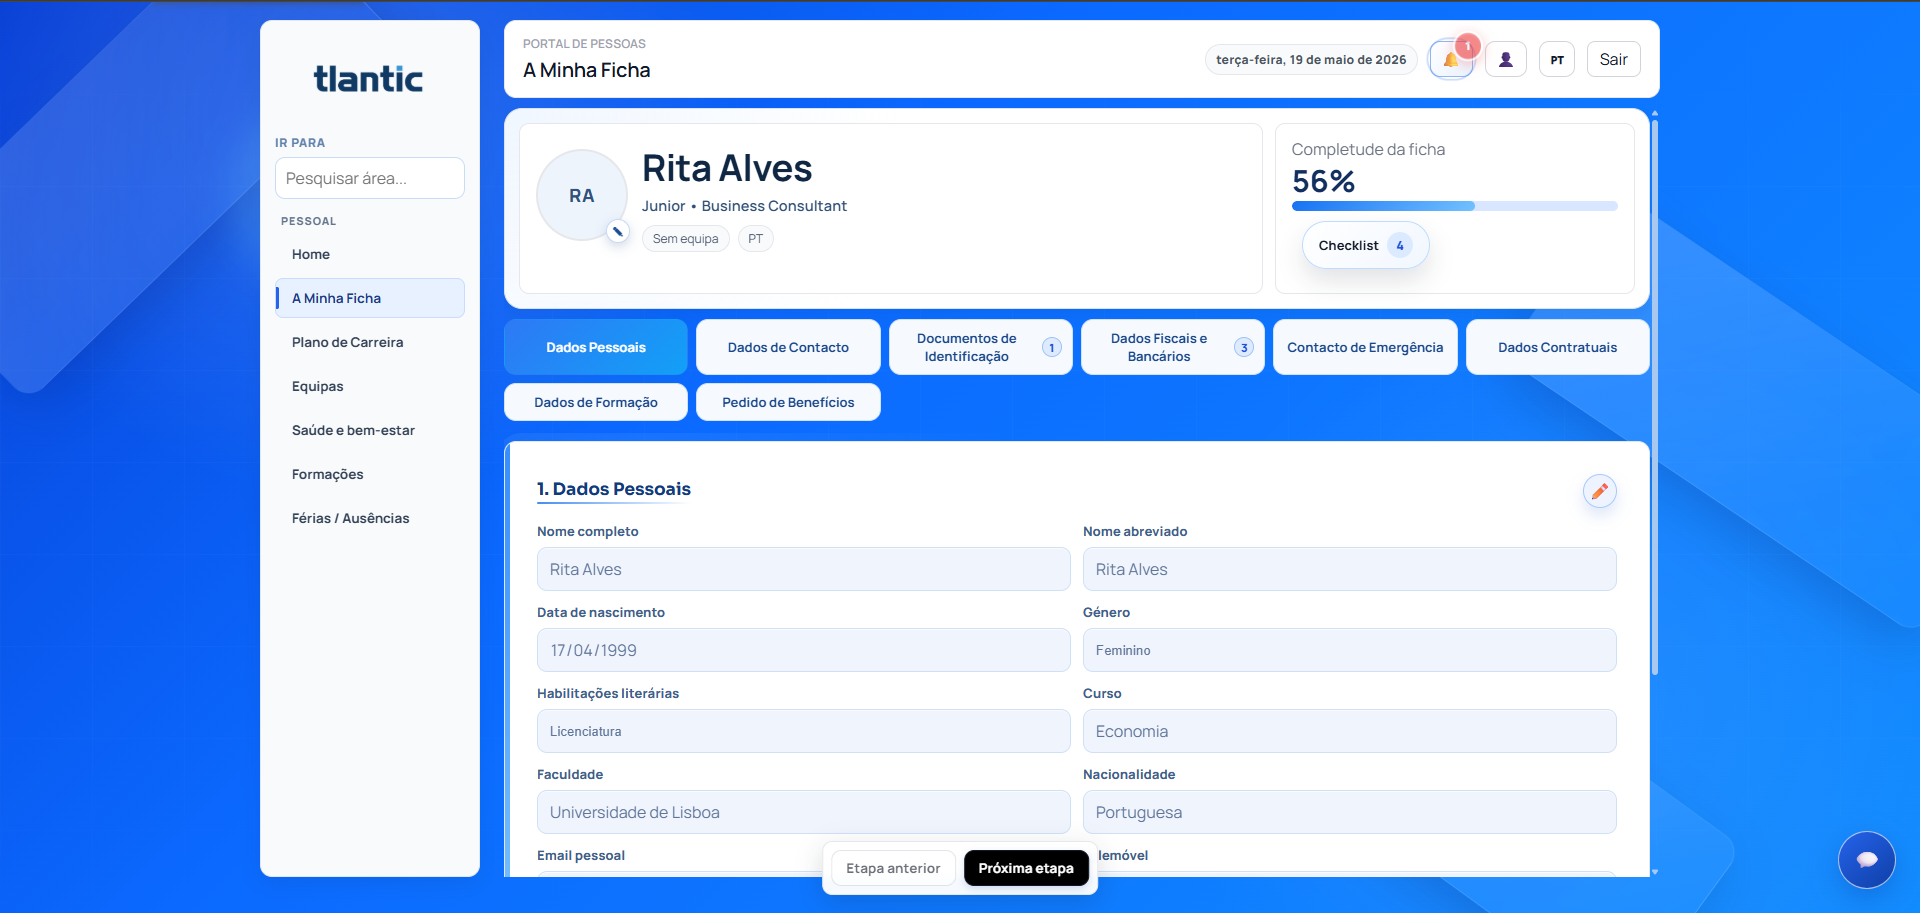
\includegraphics[width=0.94\textwidth]{screenshots/ficha.png}
  \caption{Evidência V3 - Ficha de colaborador (perfil) com dados estruturados.}
\end{figure}

\begin{figure}[htbp]
  \centering
  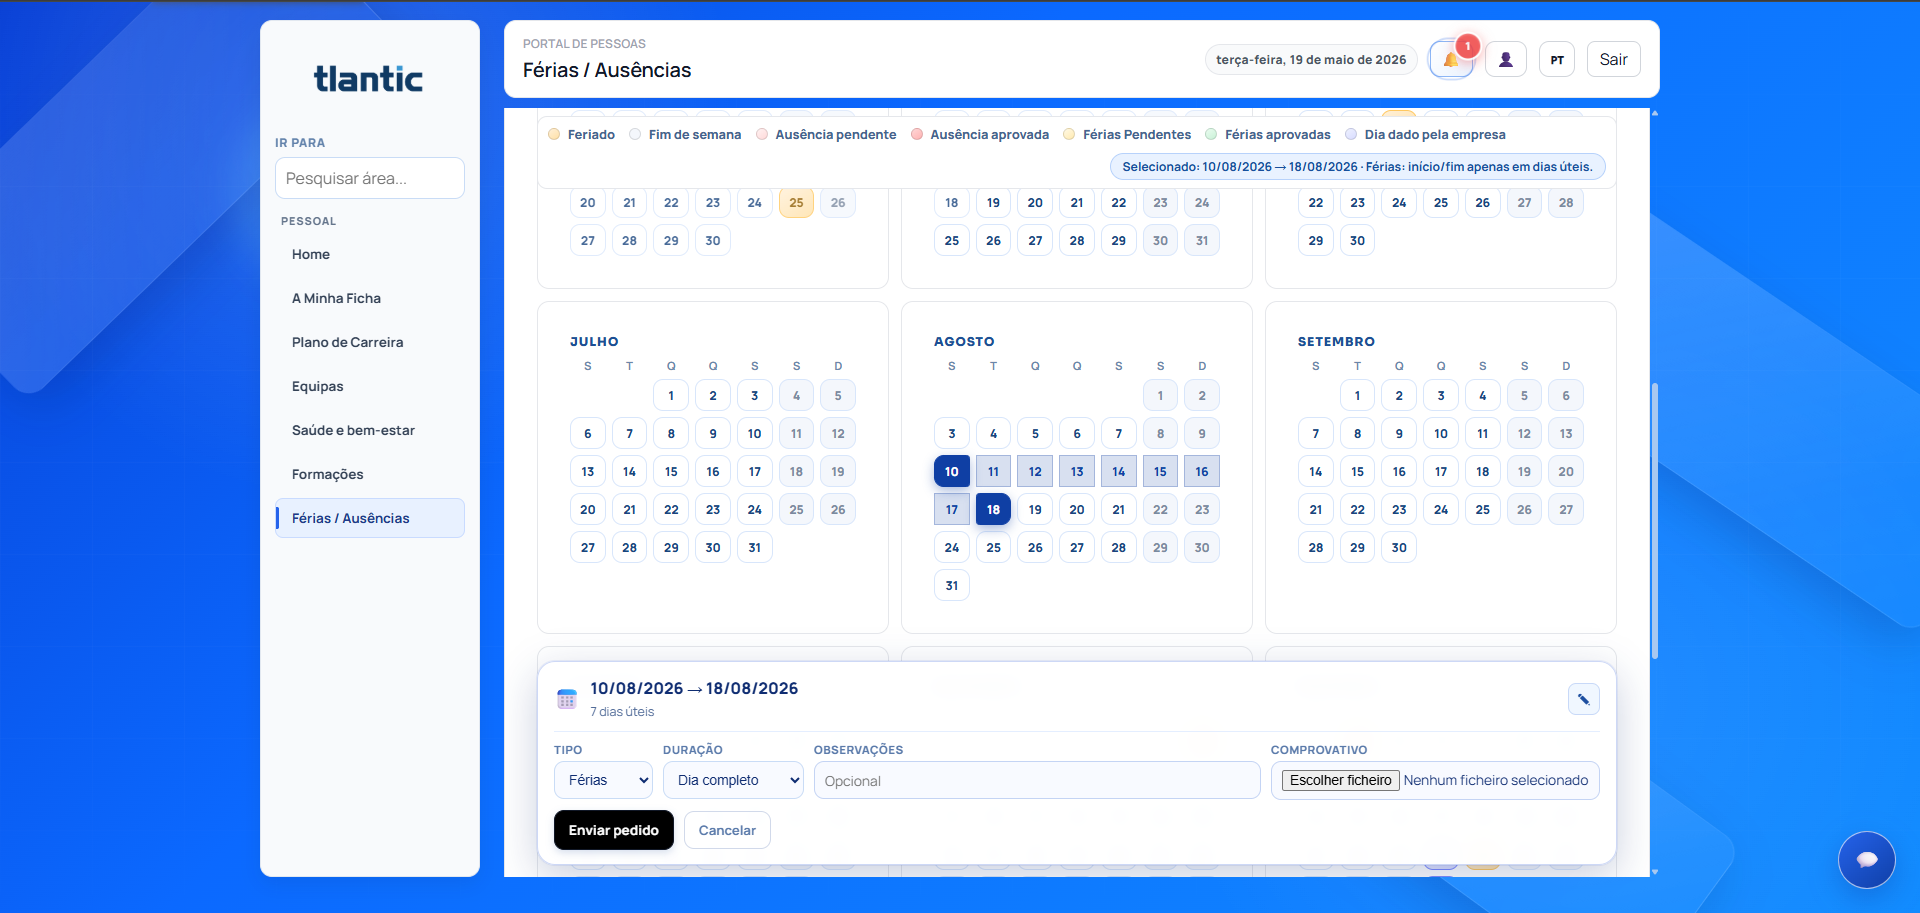
\includegraphics[width=0.94\textwidth]{screenshots/pedido_ferias.png}
  \caption{Evidência E1 - Fluxo de pedido de férias no módulo de férias/ausências.}
\end{figure}

\begin{figure}[htbp]
  \centering
  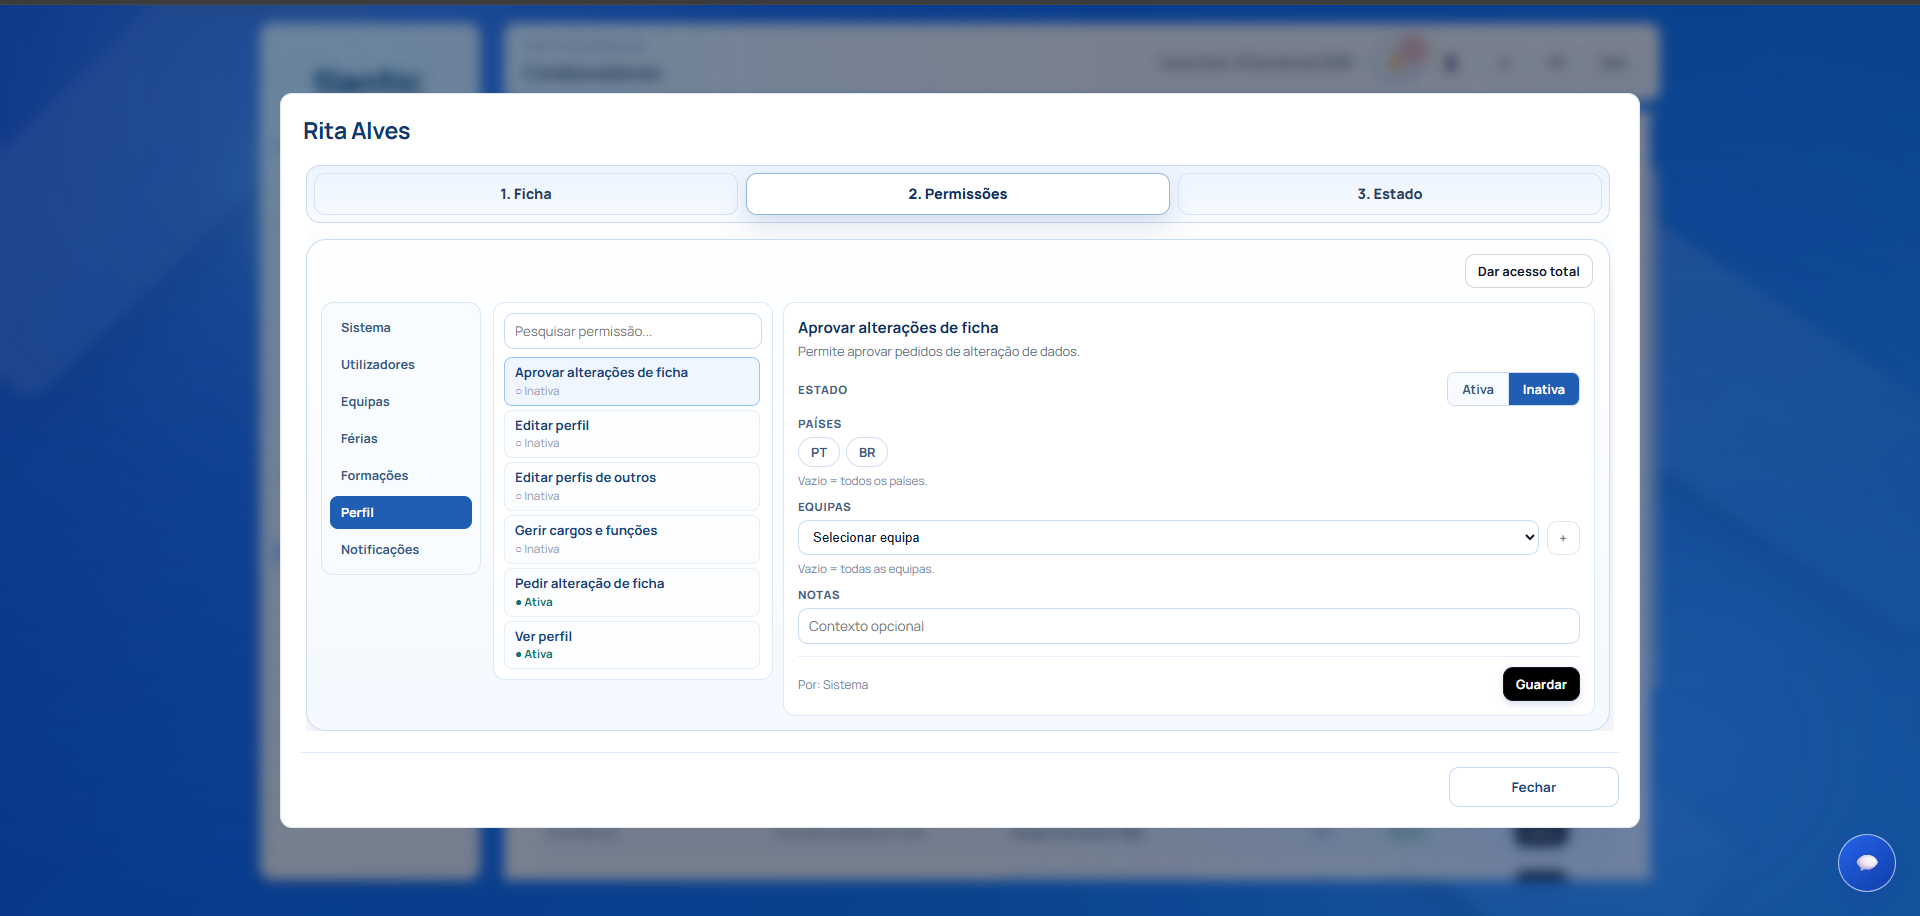
\includegraphics[width=0.94\textwidth]{screenshots/permissoes.png}
  \caption{Evidência E2 - Gestão de permissões por utilizador para governação de acessos.}
\end{figure}

\begin{figure}[htbp]
  \centering
  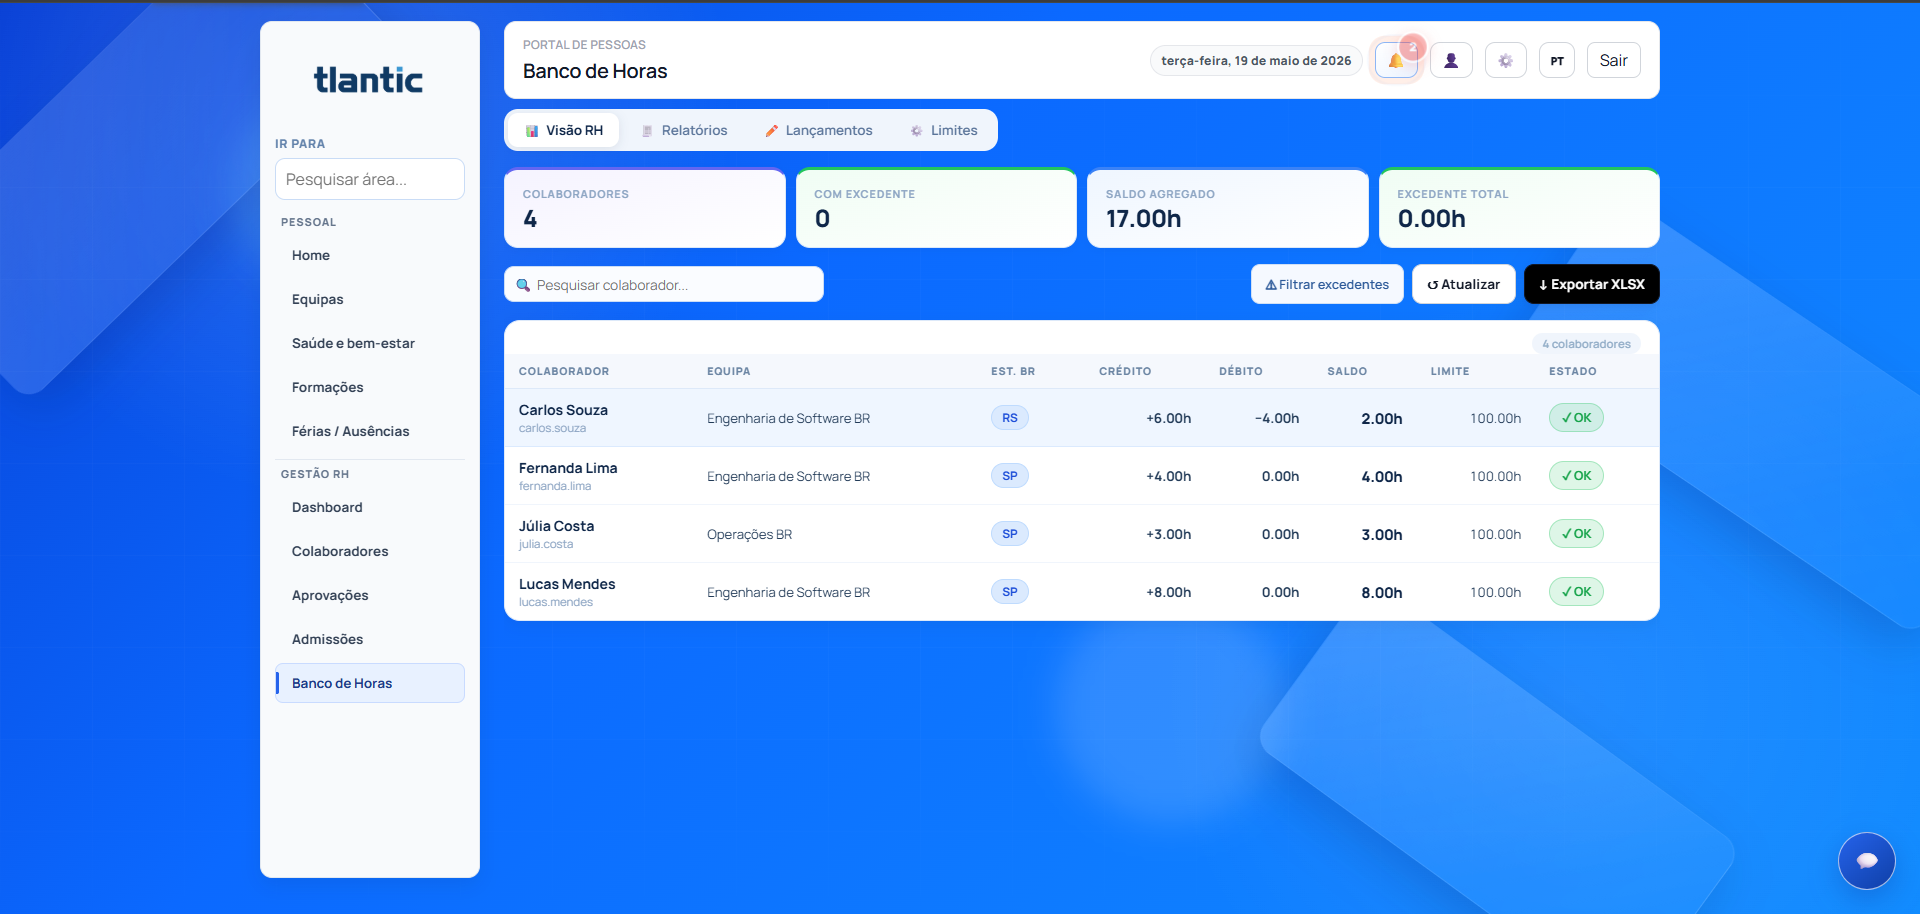
\includegraphics[width=0.94\textwidth]{screenshots/banco_horas.png}
  \caption{Evidência E3 - Banco de horas BR com consulta de saldo e movimentos.}
\end{figure}


\section{Plano com Principais Tarefas Terminadas / Em Curso}

\rowcolors{1}{ROWSHADE}{white}
\begin{longtable}{>{\small\bfseries}p{4.2cm} >{\small\centering\arraybackslash}p{2.2cm} >{\small\centering\arraybackslash}p{2.3cm} >{\small}p{4.9cm}}
\theadrow
\tH{Tarefa} & \tH{Estado} & \tH{Data de fim} & \tH{Notas} \\
\midrule
\endfirsthead
\theadrow
\tH{Tarefa} & \tH{Estado} & \tH{Data de fim} & \tH{Notas} \\
\midrule
\endhead
Fecho da análise e desenho & Completa & 22/05/2026 & Estrutura técnica validada \\
Núcleo funcional da plataforma & Completa & 22/05/2026 & Login, perfil, férias e permissões estabilizados \\
Banco de horas BR e relatório semanal & Completa & 22/05/2026 & Regras regionais já ativas \\
Admissões e plano de carreira & Completa & 22/05/2026 & Fluxos operacionais prontos \\
Cobertura de regressão E2E & Em curso & PC4 & Reforço para cenários limite \\
Refinamento de experiência e performance & Em curso & PC4 & Ajustes pós-piloto \\
\bottomrule
\end{longtable}

\section{Plano com as Fases Futuras}

\rowcolors{1}{ROWSHADE}{white}
\begin{longtable}{>{\small\bfseries}p{2.9cm} >{\small}p{3.8cm} >{\small\centering\arraybackslash}p{1.6cm} >{\small\centering\arraybackslash}p{1.6cm} >{\small\centering\arraybackslash}p{1.8cm} >{\small}p{2.0cm}}
\theadrow
\tH{Tarefa} & \tH{Descrição} & \tH{Início} & \tH{Duração} & \tH{Prioridade} & \tH{Responsável} \\
\midrule
\endfirsthead
\theadrow
\tH{Tarefa} & \tH{Descrição} & \tH{Início} & \tH{Duração} & \tH{Prioridade} & \tH{Responsável} \\
\midrule
\endhead
Consolidação pós-piloto & Correções finais e estabilização & 15/06 & 2 sem. & Elevada & Estudante \\
Expansão de regressão E2E & Cenários limite e robustez & 15/06 & 2 sem. & Elevada & Estudante \\
Refinamento de UX & Ajustes de interação e leitura & 15/06 & 2 sem. & Média & Estudante + Supervisora \\
Performance & Otimização de queries e carregamento & 20/06 & 1 sem. & Média & Estudante \\
Preparação da defesa & Narrativa final e ensaio da demo & 24/06 & 1 sem. & Elevada & Estudante + Orientador \\
\bottomrule
\end{longtable}

\section{Problemas Surgidos e Riscos}

\subsection{Problemas ativos}
\begin{itemize}
  \item A cobertura E2E ainda pode crescer em cenários de exceção.
  \item A estrutura interna do código pode ser otimizada, para facilitar a manutenção.
\end{itemize}

\subsection{Problemas resolvidos}
\begin{itemize}
  \item Atualização de permissões estabilizada após alterações de acesso total.
  \item Regras BR de férias e banco de horas fechadas e consistentes.
  \item Ciclo entre aprovação, notificação e auditoria já alinhado.
\end{itemize}

\subsection{Riscos}
\rowcolors{1}{ROWSHADE}{white}
\begin{longtable}{>{\small\bfseries}p{0.9cm} >{\small}p{6.0cm} >{\small}p{5.9cm}}
\theadrow
\tH{ID} & \tH{Risco} & \tH{Mitigação} \\
\midrule
\endfirsthead
\theadrow
\tH{ID} & \tH{Risco} & \tH{Mitigação} \\
\midrule
\endhead
R1 & Regressão em regras PT/BR após ajustes de interface & Testes de regressão por domínio antes de cada entrega \\
R2 & Sobrecarga de escopo perto da defesa & Congelamento de escopo por checkpoint \\
R3 & Feedback de negócio em atraso & Janela dedicada de validação com stakeholders \\
R4 & Divergência entre documento e implementação & Revisão cruzada entre TEX, Gantt e evidência técnica \\
\bottomrule
\end{longtable}
\section{Conclusão}

\begin{callout}
O PC3 entrega um sistema funcionalmente preparado para piloto operacional, com rastreabilidade de decisão, controlo de acesso e regras de negócio ativas.
\end{callout}

\section{Ficheiros da Entrega PC3}

\begin{itemize}
  \item \texttt{PROES\_2025\_2026\_PC3.pptx}
  \item \texttt{PROES\_PC3\_2025\_2026.tex}
  \item \texttt{ESPECIFICACAO\_FUNCIONAL\_SMARTER\_HUB\_PC3.tex}
  \item \texttt{gantt\_chart\_pc3.xlsx}
\end{itemize}

\appendix
\section{Anexo A - Diagramas de Suporte}

\begin{figure}[htbp]
  \centering
  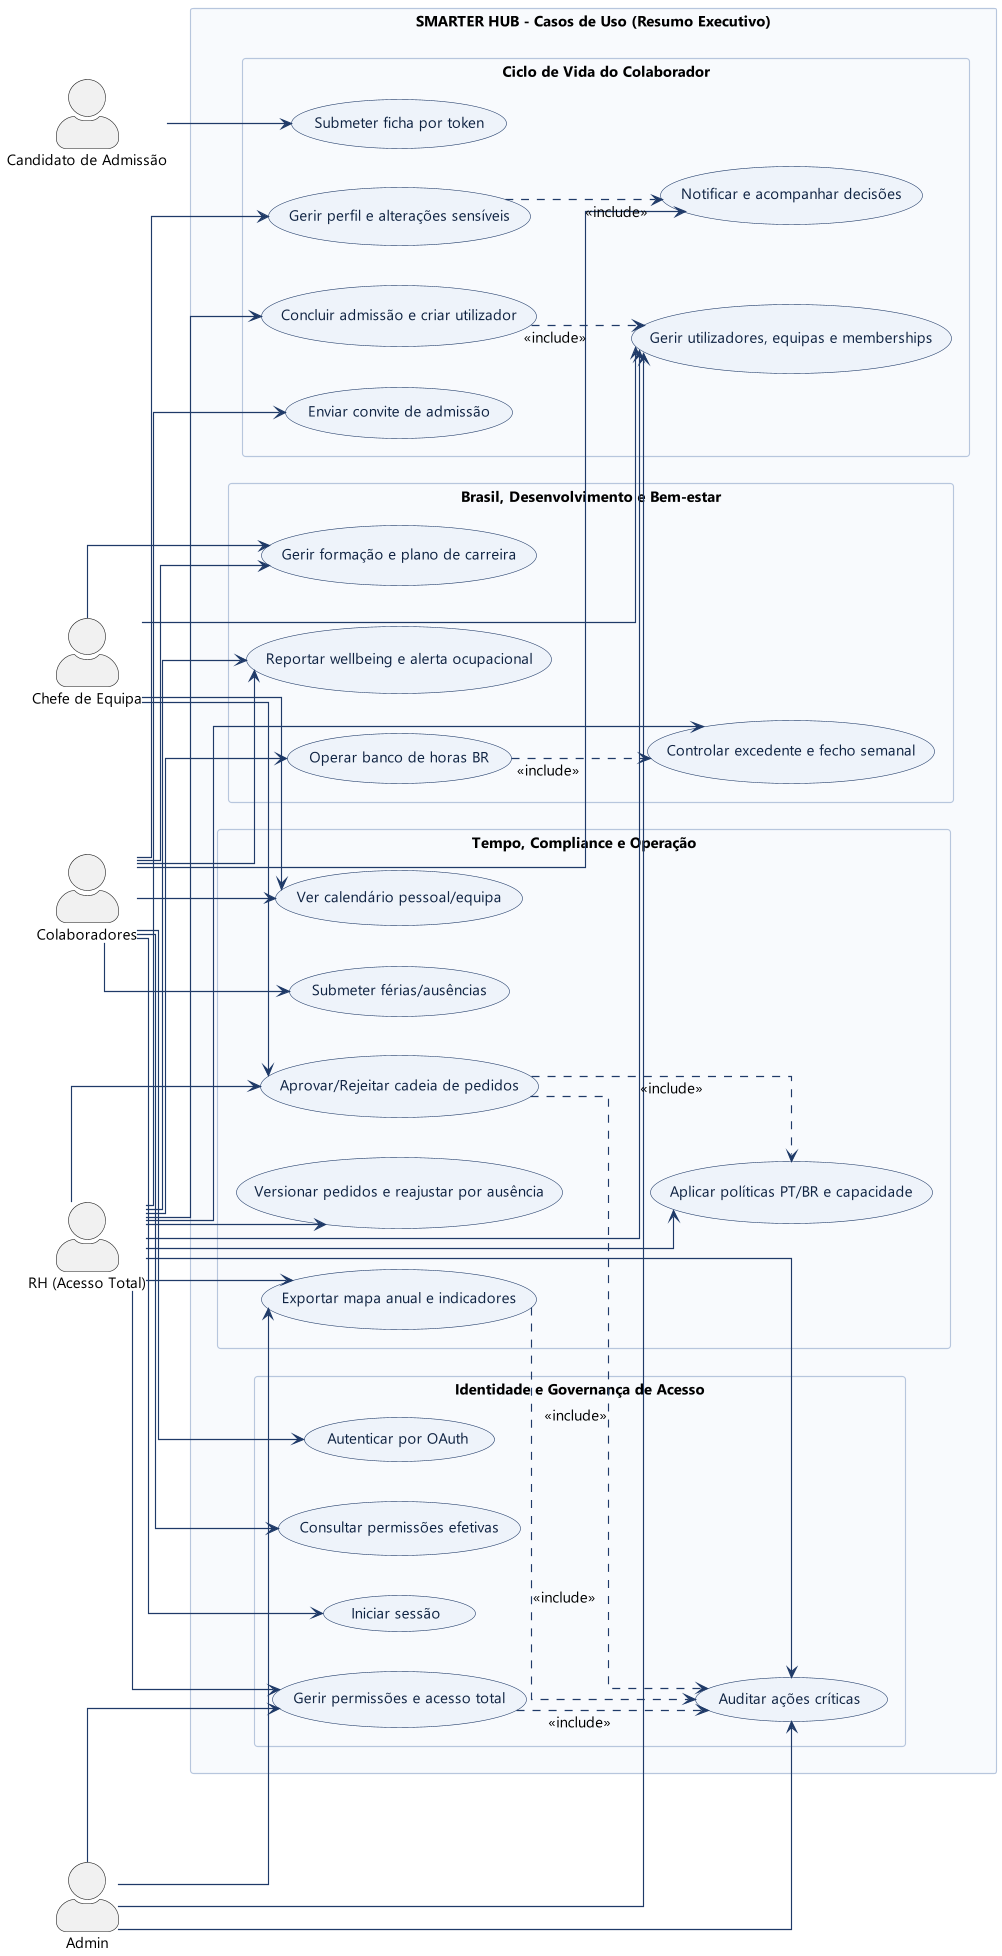
\includegraphics[width=0.94\linewidth]{../../out/docs/PC3/diagramas/01-diagrama-casos-de-uso-resumo/smarter_hub_casos_de_uso_resumo.png}
  \caption{Casos de uso do SMARTER HUB (versão resumida).}
  \label{fig:anexo-casos-uso}
\end{figure}

\begin{figure}[htbp]
  \centering
  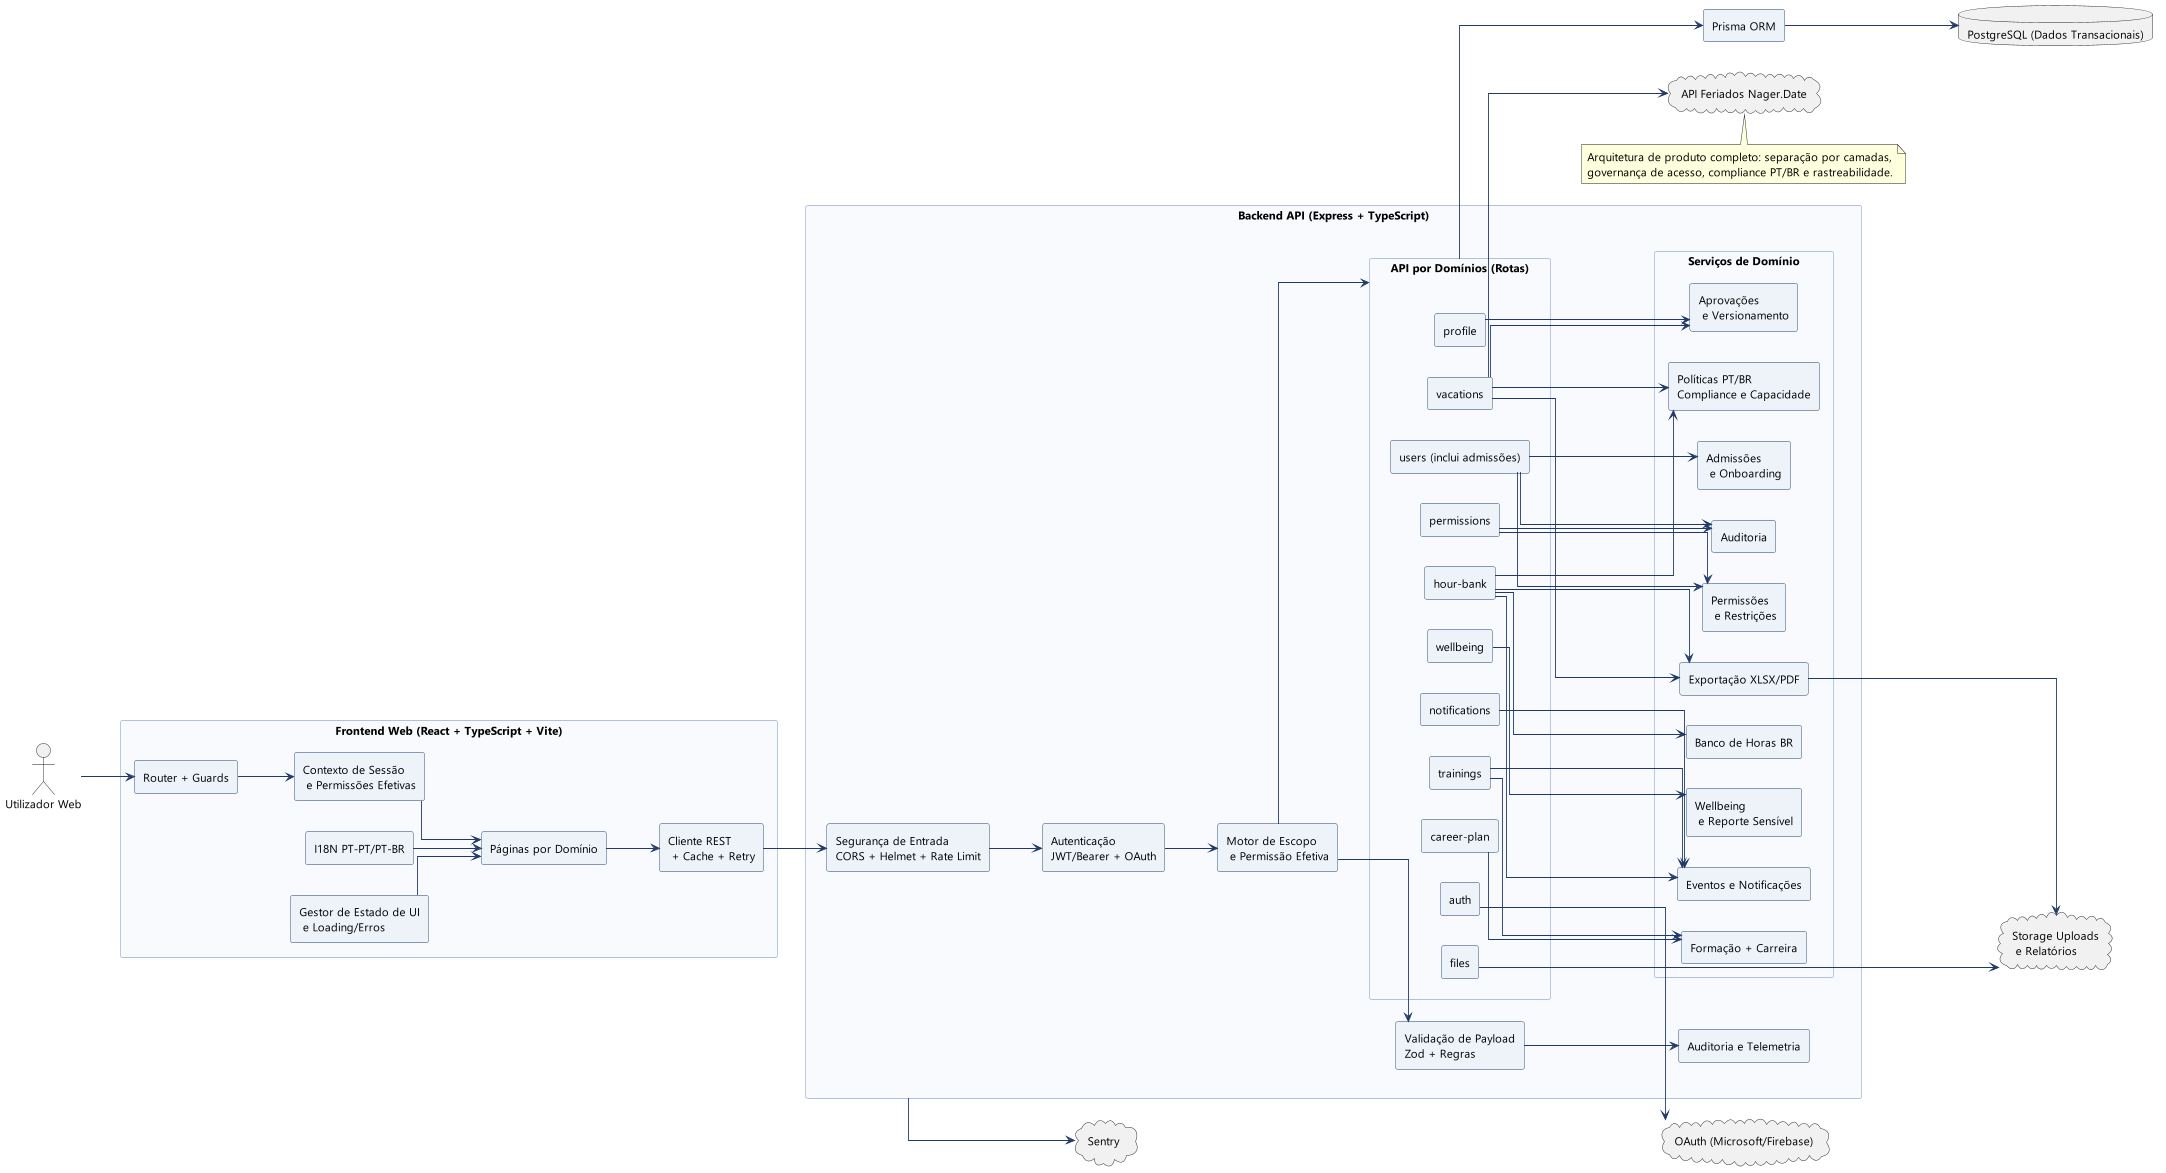
\includegraphics[width=0.94\linewidth]{../../out/docs/PC3/diagramas/02-diagrama-arquitetura-componentes/smarter_hub_arquitetura_completa.png}
  \caption{Arquitetura por componentes do SMARTER HUB (versão completa).}
  \label{fig:anexo-arquitetura}
\end{figure}

\begin{figure}[htbp]
  \centering
  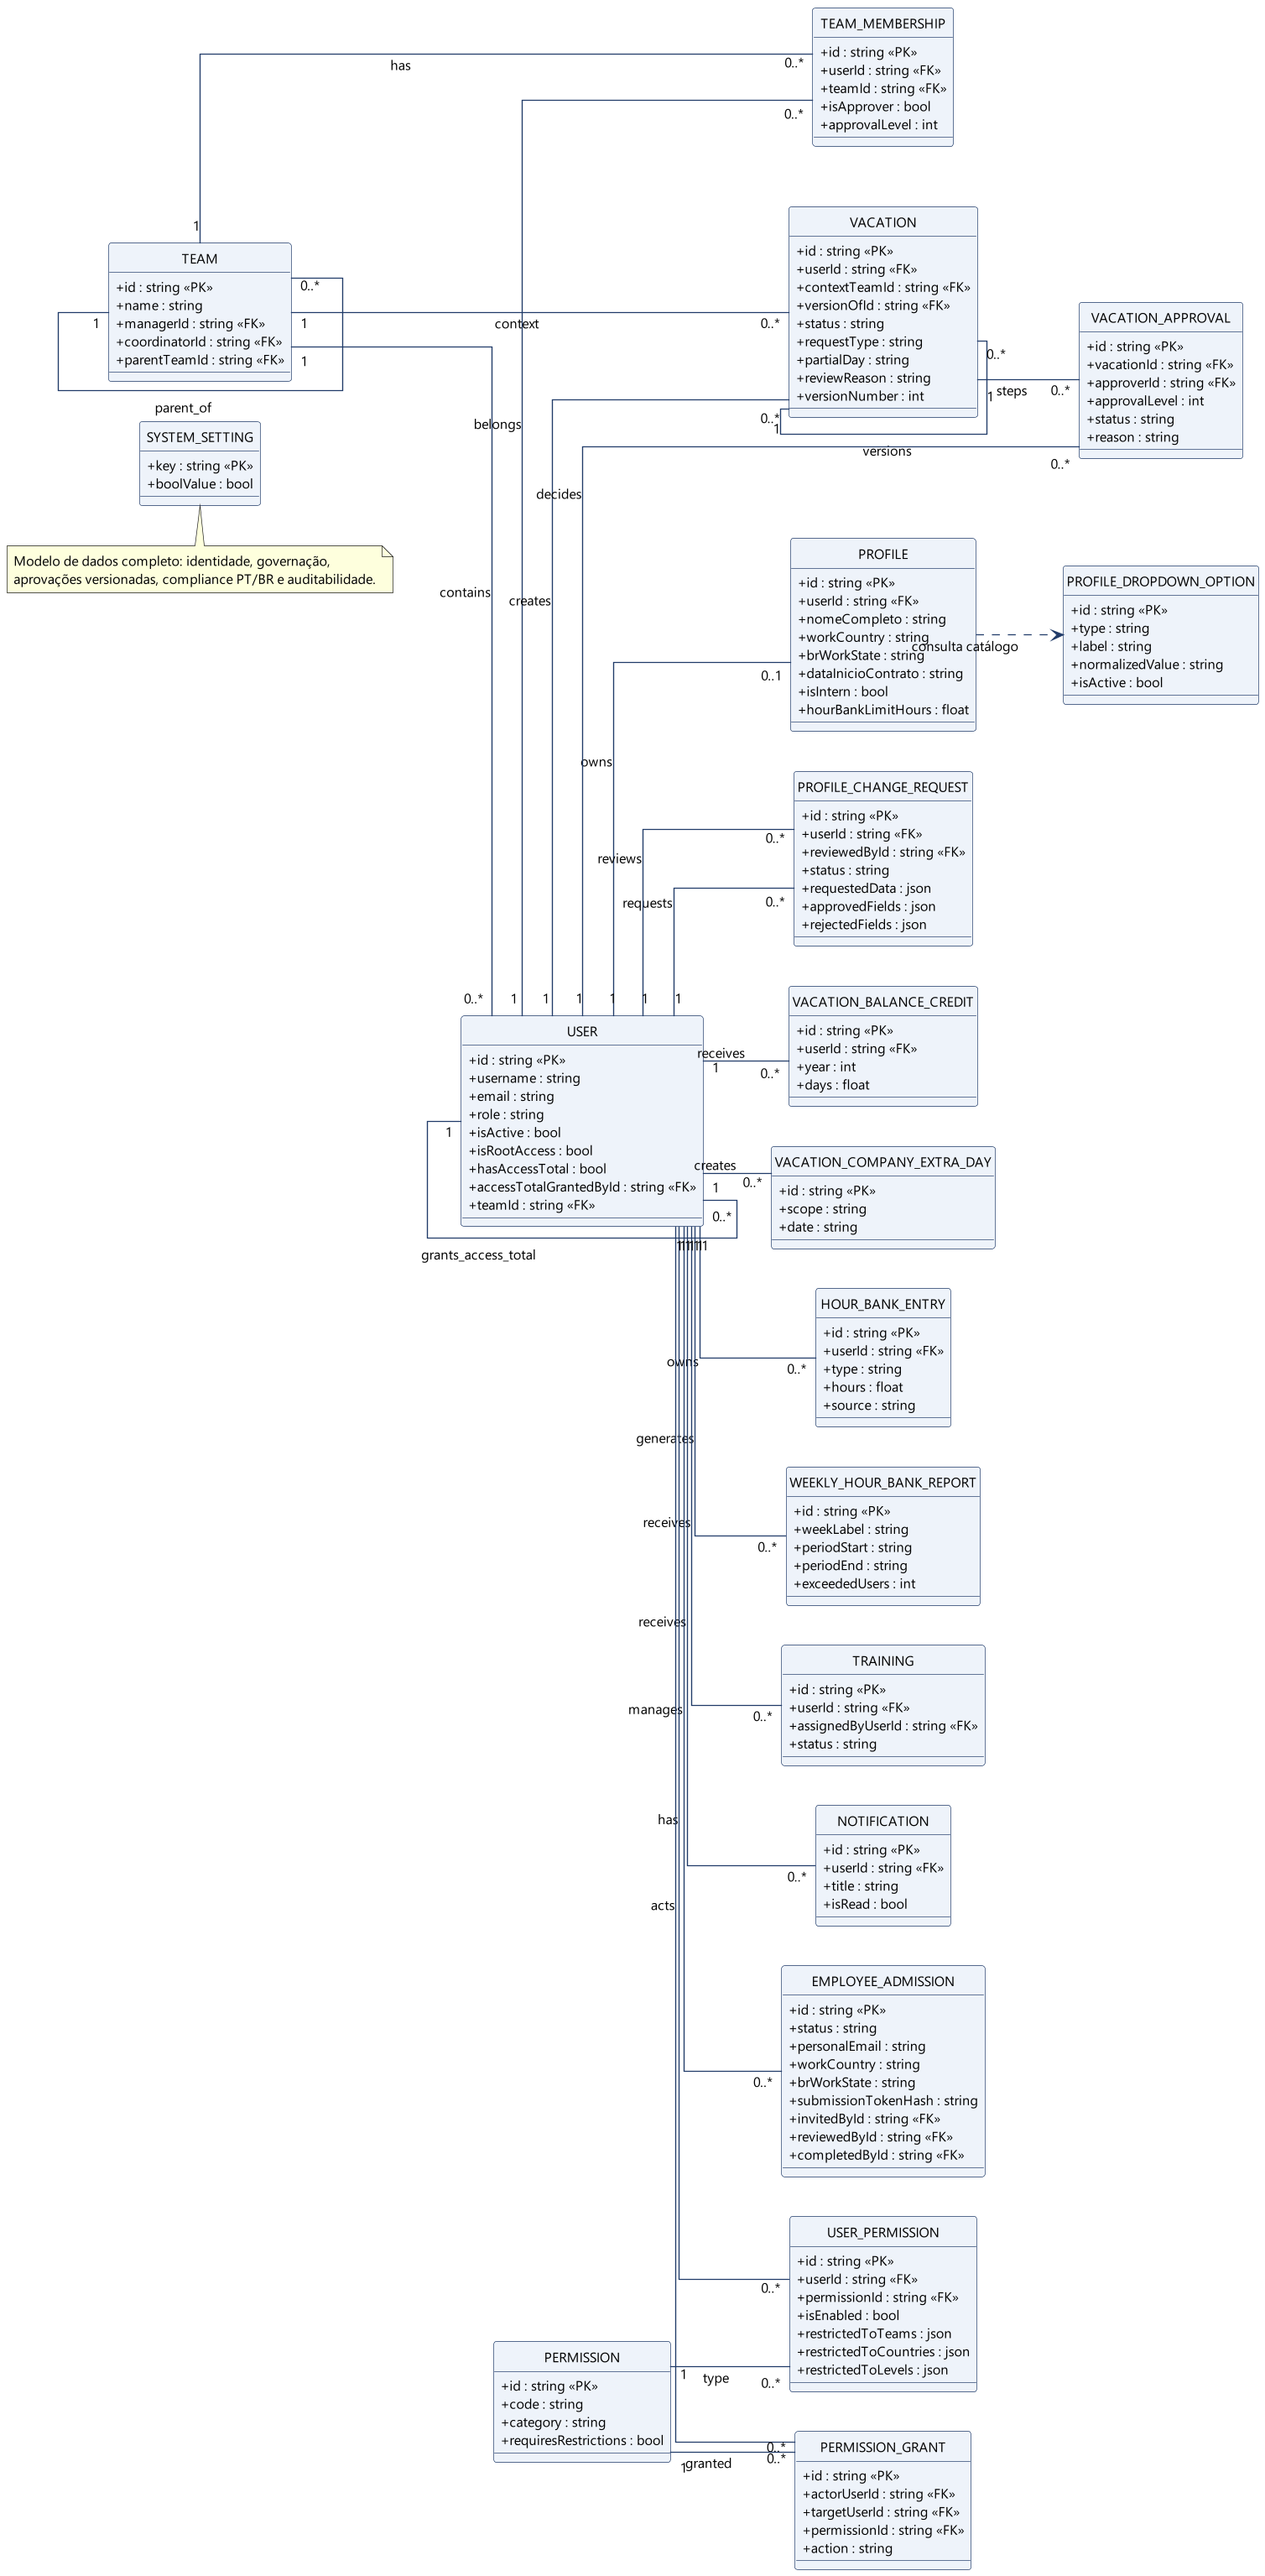
\includegraphics[width=0.94\linewidth]{../../out/docs/PC3/diagramas/04-diagrama-classes-modelo-dados/smarter_hub_modelo_dados_completo.png}
  \caption{Diagrama de classes do modelo de dados do SMARTER HUB (versão completa).}
  \label{fig:anexo-modelo-dados}
\end{figure}

\end{document}
